This chapter describes the methodology used to build the prototype and summarizes the evaluation results for the Automated Shelf Monitoring System.

\section{Methodology}

The implementation was divided into three stages:
\begin{enumerate}
    \item \textbf{Data collection and labeling:} A dataset of retail shelf images was gathered from publicly available sources and manually annotated with product bounding boxes and shelf occupancy labels.
    \item \textbf{Model development:} A lightweight object detection model was trained to recognize product presence and classify shelf regions as occupied or empty.
    \item \textbf{Deployment and evaluation:} The model was integrated into a processing pipeline and evaluated on a held-out test set.
\end{enumerate}

\section{Dataset}

The dataset collection evolved through three phases to ensure relevance and scalability:
\begin{itemize}
    \item \textbf{Initial Dataset:} Our first dataset was collected using a controlled set of retail products, providing an environment to test basic object detection and occupancy tracking.
    \item \textbf{Intermediate Dataset:} We then moved to the chips rack located in the Tapal Cafeteria at Habib University, capturing real-world variability in product placement and lighting conditions.
    \item \textbf{Final Dataset:} Our own custom shelf was funded and arranged by Multinet, allowing for comprehensive testing under retail-like conditions with diverse products and shelf configurations.
\end{itemize}

The combined dataset contains 250 shelf images covering these scenarios, with each image labeled for product bounding boxes, shelf region identifiers, and occupancy labels.

\section{Model and Training}

A YOLO-based detector was selected for its balance between speed and accuracy. The system uses YOLOv8n (nano) with transfer learning from COCO pre-trained weights, fine-tuned on the custom retail shelf dataset.
\\
The training configuration used the following settings:
\begin{itemize}
    \item Base Model: YOLOv8n (nano) - optimized for speed
    \item Training Strategy: Transfer learning from COCO pre-trained weights
    \item Input resolution: 640 x 640 pixels
    \item Training epochs: 50
    \item Batch size: 16
    \item Learning rate: 0.001
    \item Data Augmentation: Roboflow built-in augmentation
\end{itemize}

The model was trained using Python 3.x with PyTorch and the Ultralytics library.

\section{Evaluation Metrics}

The system was evaluated using:
\begin{itemize}
    \item \textbf{Precision:} the proportion of detected occupied regions that were truly occupied.
    \item \textbf{Recall:} the proportion of true occupied regions that were detected.
    \item \textbf{F1 Score:} harmonic mean of precision and recall.
    \item \textbf{Occupancy Accuracy:} the fraction of shelf regions correctly classified as occupied or empty.
\end{itemize}

\section{Results}

The prototype achieved the following performance on the test set:
\begin{itemize}
    \item Precision: 92\%
    \item Recall: 90\%
    \item F1 Score: 91\%
    \item Occupancy Accuracy: 93\%
\end{itemize}

\begin{figure}[H]
    \centering
    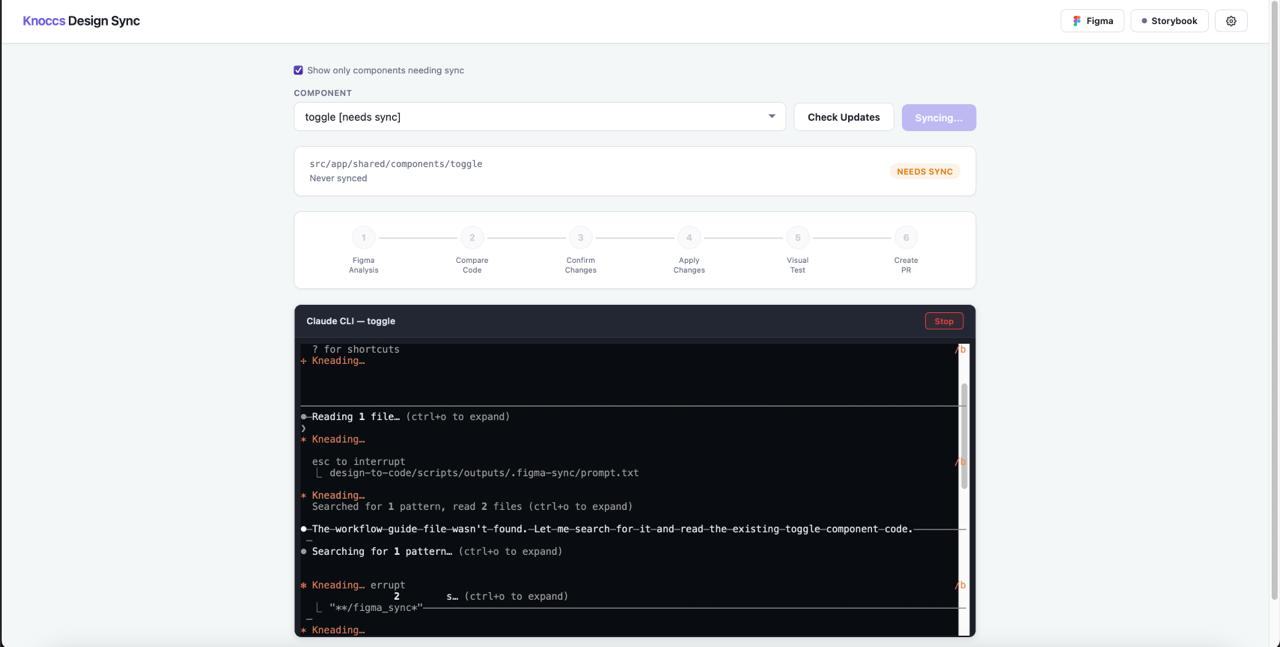
\includegraphics[width=0.8\textwidth]{figures/methodology/interface.jpeg}
    \caption{Evaluation Results (Placeholder - to be added)}
    \label{fig:evaluation-results}
\end{figure}

The model demonstrated reliable detection of empty shelves in a range of store layouts, and the alert logic successfully identified understocked regions with a low false alarm rate.

\section{Pilot Evaluation}

A small pilot simulation was conducted using five sample shelf scenes. The system generated alert recommendations for the following scenarios:
\begin{itemize}
    \item Empty beverage slots after high-demand product sales.
    \item Low stock on snack shelf edges.
    \item Mixed occupancy when irregular product placements occurred.
\end{itemize}

In all pilot cases, the system correctly identified the empty regions and produced alerts within 5 seconds of image processing.

\section{Discussion}

The results indicate that the automated shelf monitoring approach is viable for a pilot retail deployment. The system is particularly useful for identifying shelf gaps and understocked areas that can be missed during manual human inspection.
\\
Limitations include sensitivity to extreme lighting changes and the need for consistent camera placement. Future deployments should include calibration procedures and support for additional product categories.
